\chapter{Coordinate Transform}
\label{ch:transform}

Open from \uipth{2.\ Preprocess $\to$ Transform / Align\ldots}.

\begin{warnbox}
Transforms modify the dataset \textbf{in memory} and cannot be undone. If you make a mistake, click \uipth{Reload Last Dataset} in the sidebar to reload from disk and start again.
\end{warnbox}

In PIV experiments, the camera is rarely perfectly aligned with the flow geometry. Even a $1^\circ$ tilt introduces errors in all derived quantities, including mean profiles, Reynolds stresses, line profiles, and integral scales. Always apply the transform \emph{before} opening any analysis module.

\begin{figure}[htbp]
  \centering
  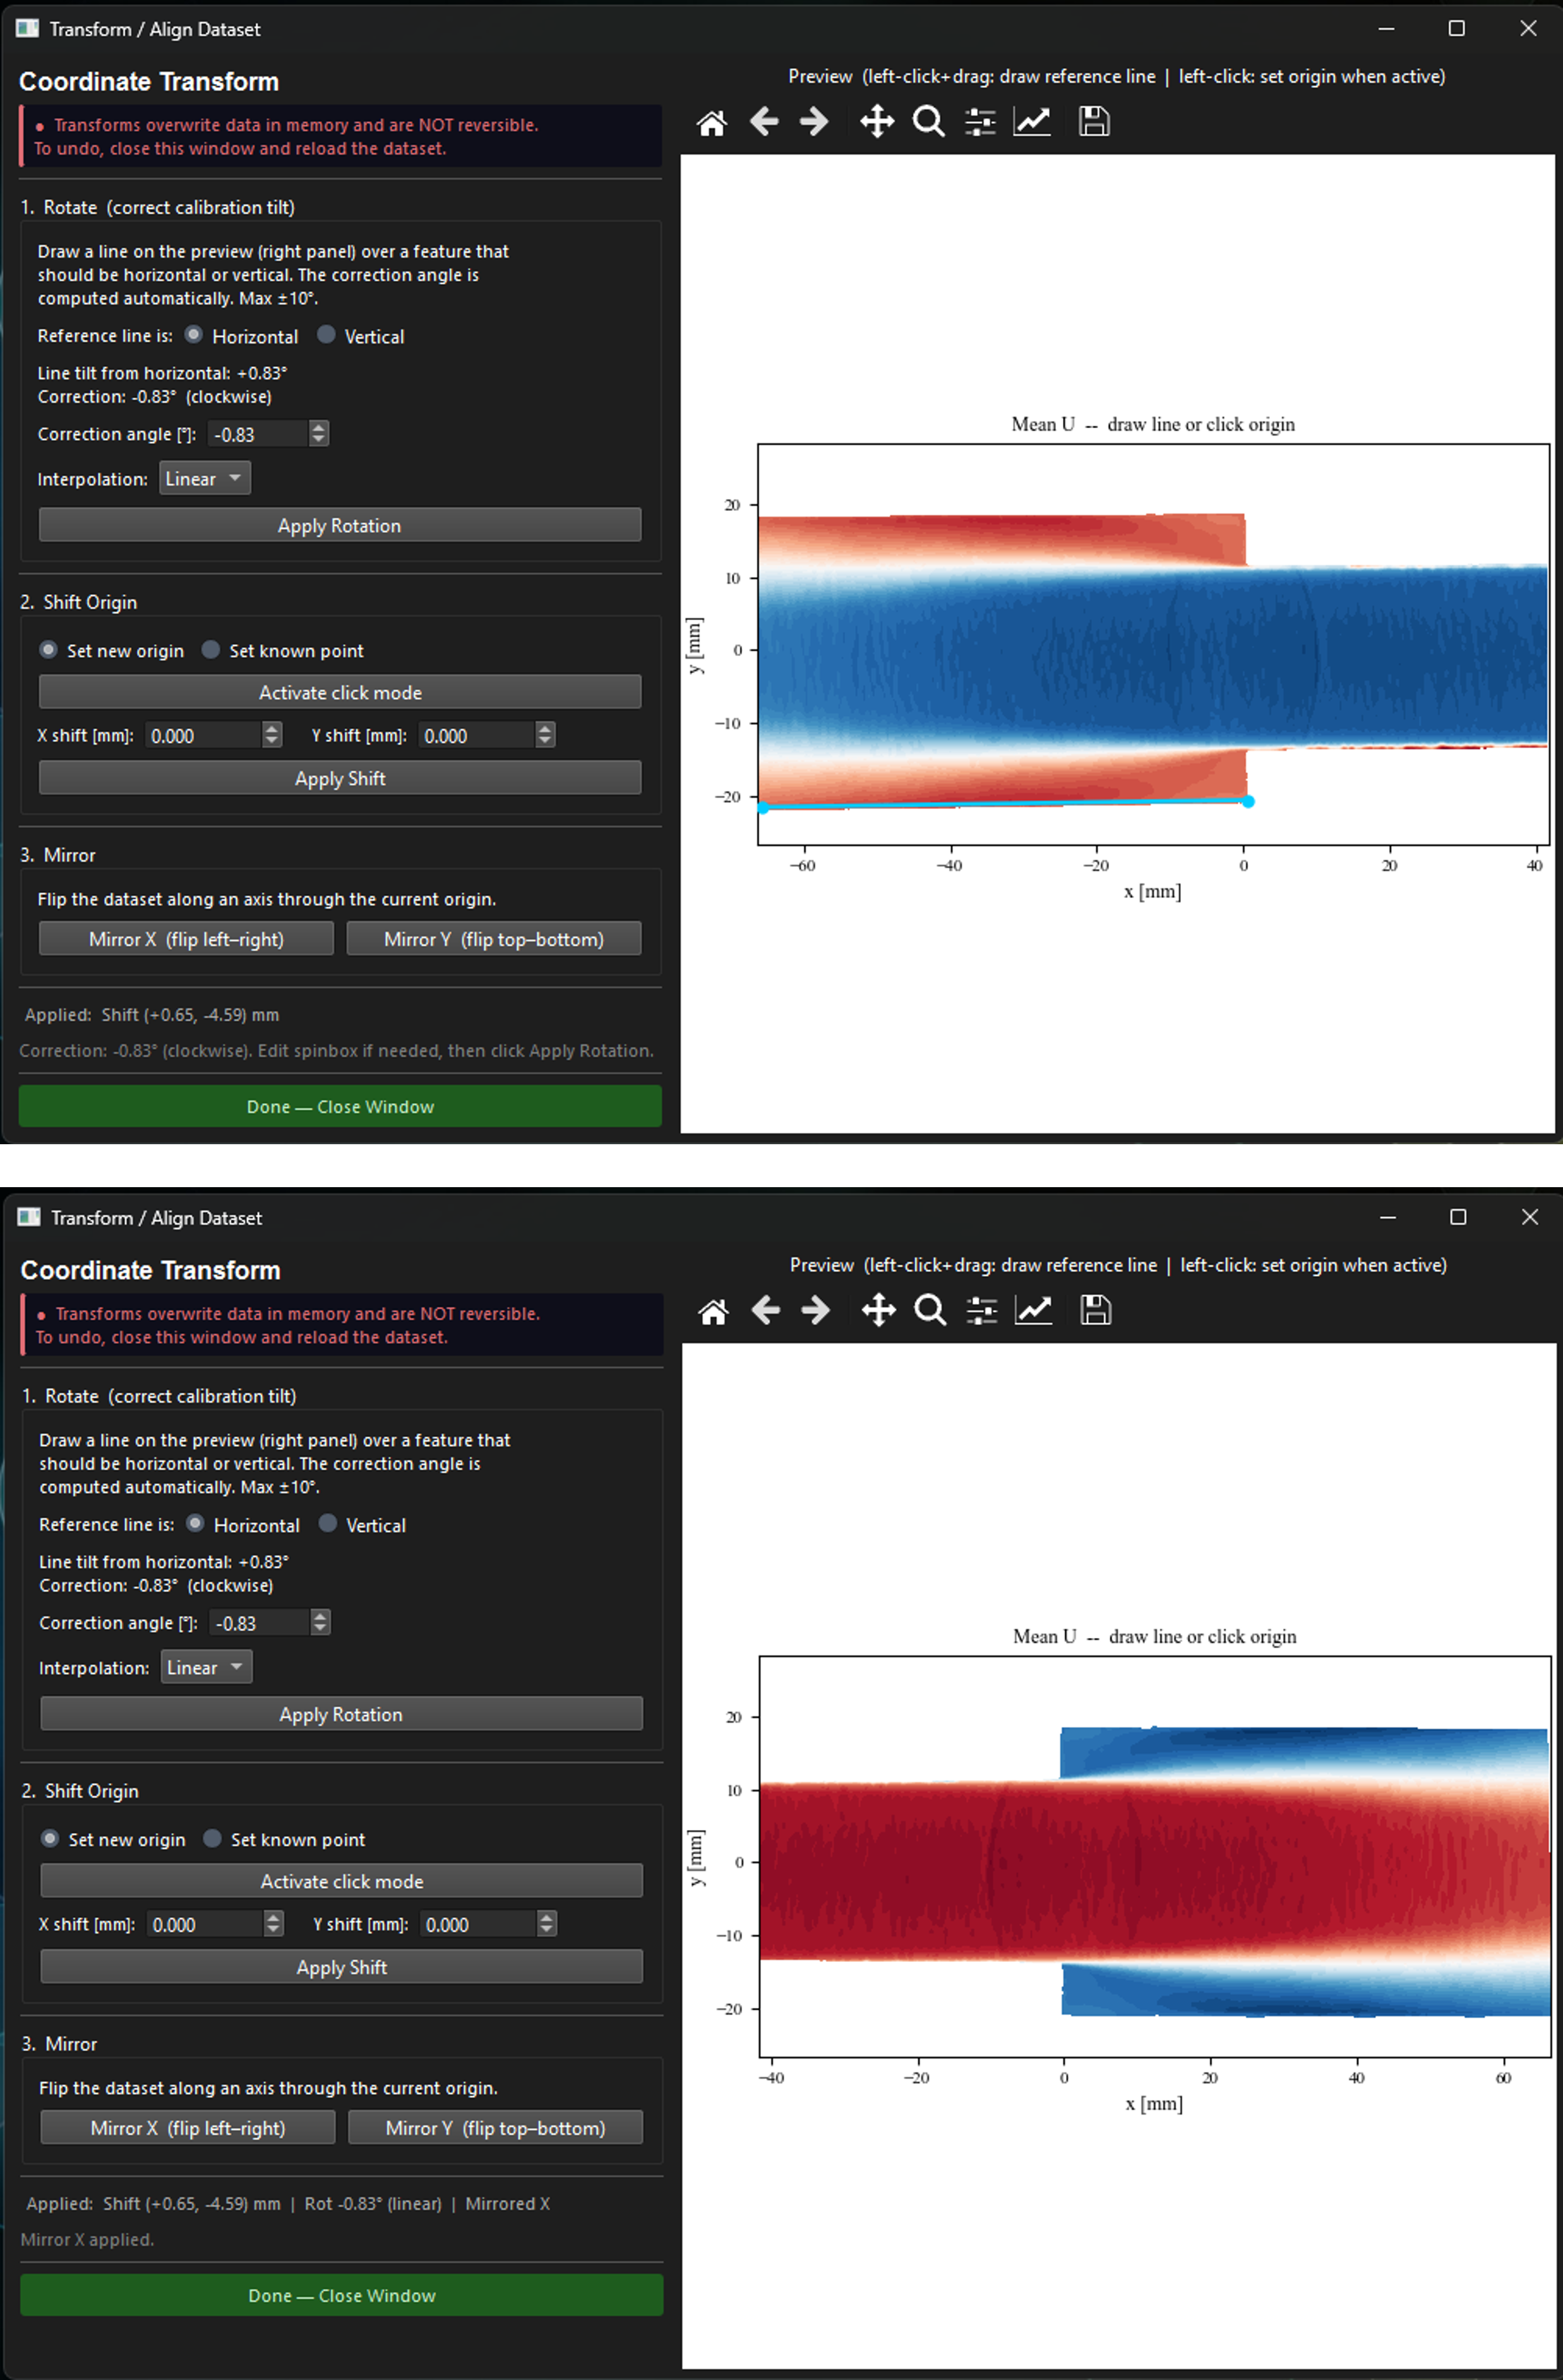
\includegraphics[width=0.92\linewidth]{fig11}
  \caption{Coordinate Transform window. Left: controls. Right: live preview of the mean field. A reference line drawn along the lower pipe wall is shown in cyan. The computed correction angle appears automatically in the left panel.}
  \label{fig:transform}
\end{figure}

\section{Rotation}

\begin{stepbox}
\begin{enumerate}[leftmargin=1.5em, topsep=2pt]
  \item Left-click and drag on the field preview to draw a reference line along any feature that should be perfectly horizontal or vertical (wall, step edge, pipe centerline).
  \item The misalignment angle is computed automatically and shown in the \uipth{Correction angle} field.
  \item Choose \uipth{Linear} (fast) or \uipth{Cubic} (smoother, recommended for final results).
  \item Click \uipth{Apply Rotation}.
\end{enumerate}
\end{stepbox}

\begin{notebox}
Rotation is limited to $\pm10^\circ$. For larger corrections, fix the calibration in DaVis and re-export your data.
\end{notebox}

\section{Origin shift}

Moves the coordinate origin $(0, 0)$ to a physically meaningful reference point such as a step corner, pipe inlet, or cylinder center. Two modes are available: \uipth{Set new origin} (click on the point that should become $(0, 0)$) and \uipth{Set known point} (click a point and enter what its real-world coordinates should be).

\section{Mirror}

Flips the entire dataset along an axis through the current origin. \uipth{Mirror X} negates all $x$-coordinates and the $U$ component; \uipth{Mirror Y} negates all $y$-coordinates and the $V$ component.

% ============================= CHAPTER 4 ==============================
